%ACM journals format:
\documentclass[prodmode,acmtodaes]{acmsmall} 
\usepackage[ruled]{algorithm2e}
\renewcommand{\algorithmcfname}{ALGORITHM}
\SetAlFnt{\small}
\SetAlCapFnt{\small}
\SetAlCapNameFnt{\small}
\SetAlCapHSkip{0pt}
\IncMargin{-\parindent}

%Springer DAES format below:
%\documentclass[runningheads,a4paper]{llncs}
%\usepackage{amssymb}
%\setcounter{tocdepth}{3}
%\usepackage{graphicx}

% Metadata Information
%\acmVolume{9}
%\acmNumber{4}
%\acmArticle{39}
%\acmYear{2010}
%\acmMonth{3}

% Document starts
\begin{document}

% Page heads
\markboth{I. Filippopoulos et al.}{Data Interleaving and Memory Mapping on VLIW architectures}

% Title portion
\title{Integrated Optimization Methodology for Data Interleaving and Memory Mapping Exploration on VLIW architectures}
\author{IASON FILIPPOPOULOS
\affil{Norwegian University of Science and Technology}
NAMITA SHARMA 
\affil{Indian Institute of Technology Delhi}
FRANCKY CATTHOOR
\affil{IMEC}
PER GUNNAR KJELDSBERG
\affil{Norwegian University of Science and Technology}
PREETI PANDA
\affil{Indian Institute of Technology Delhi}
}

\begin{abstract}
This work presents a methodology for efficient exploration of data interleaving and data-to-memory mapping options for SIMD (Single Instruction Multiple Data) platform architectures.
The system architecture includes VLIW (Very Long Instruction Word) function units and a reconfigurable clustered memory. 
The scope is the reduction of the overall energy consumption by increasing the utilization of the function units and decreasing the number of memory accesses.
The presented methodology is tested using a number of benchmark applications with irregularities on their access scheme.
Potential gains are calculated based on the energy models both for the processing and the memory part of the system.
\end{abstract}

\category{D.2.2}{Design Tools and Techniques}{Design, Methodologies}
\category{B.7.1}{Types and Design Styles}{Memory Technologies, Design}
\category{B.8.2}{Performance Analysis and Design Aids}{}

\terms{Design, Algorithms, Performance}

\keywords{Data interleaving, single instruction multiple data (SIMD), system scenarios, design space exploration, memory reconfiguration}

%\acmformat{Iason Filippopoulos, Namita Sharma, Francky Catthoor, Per Gunnar Kjeldsberg, Preeti Panda, 2015. Integrated Optimization Methodology for Data Interleaving and Memory Mapping Exploration on VLIW architectures.}

%\begin{bottomstuff}
%Author's addresses: Iason Filippopoulos {and} Per Gunnar Kjeldsberg, Department of Electronics and Telecommunications, Norwegian University of Science and Technology (NTNU), Trondheim, Norway; Namita Sharma  {and} Preeti Panda, Department of Computer Science and Engineering, Indian Institute of Technology Delhi, New Delhi, India; Francky Catthoor, IMEC, Leuven, Belgium.
%\end{bottomstuff}

\maketitle

\section{Introduction}

The goal of this work is to improve both the performance and the energy consumption for data intensive applications. 
We focus on single instruction, multiple data (SIMD) architectures and deal with applications that have irregularities on their access scheme. 
SIMD architectures can potentially increase the performance of an application, providing that the utilization of them is high. 
However, applications with irregular access patterns do not provide compact sequences of data that are suitable for high utilization. 
Hence the performance is lower than expected. 
In order to improve the performance a systematic exploration of the interleaving options for application's data is needed. 

The energy consumption can be divided into two parts, namely the processing and the memory subsystem. 
The energy needed for processing depends mainly on the utilization of the FUs and any potential stalls, if the memory cannot provide data on the needed rate.
The interleaving exploration can increase the utilization of the processing subsystem and reduce time penalties for data loading.   
The energy consumption on the memory subsystem is affected by the number of memory accesses and the energy per access. 
Again, the memory architecture and the data-to-memory mapping decisions have a great impact on both the number of accesses and the energy per access.

\section{Motivational Example}

A large number of papers have demonstrated the importance of the memory organization to the overall system energy consumption. 
As shown in \cite{Gonzalez1996} memory contributes around 40\% to the overall power consumption in general purpose systems. 
Especially for embedded systems, the memory subsystem accounts for up to 50\% of the overall energy consumption \cite{Che09} and the cycle-accurate simulator presented in \cite{Ben99} estimates that the energy expenditures in the memory subsystem range from 35\% up to 65\% for different architectures. 
The breakdown of power consumption for a recently implemented embedded system presented in \cite{Hul11} shows that the memory subsystem consumes more than 40\% of the leakage power on the platform. 
According to \cite{tcm}, conventional allocation and assignment of data done by regular compilers is suboptimal. 
Performance loss is caused by stalls for fetching data and data conflicts for different tasks, due to the limited size of memory and the competition between tasks. 

To illustrate the sub-optimal utilization of SIMD architectures using conventional allocation and assignment of data, the simple example of Alg.~\ref{alg:motivation} is used.
In this example, we assume that the desired result is always the sum of 4 elements from arrays \textit{A, B, C and D}. 
The access pattern shows an irregularity, as a result of the iteration index.
For every group of four sequential array elements, there is only one used for the calculation of the result and the other three are skipped.
An intuitive interleaving optimization is the interleaving of the arrays \textit{A, B, C and D}, in order to generate sequences of elements that are all useful on the calculation of the \textit{result} variable. 
A full interleaving exploration could reveal several options to produce larger sequences of array elements that are needed during the execution of Alg.~\ref{alg:motivation}.
For example, the interleaving of every fourth line within the combined array ($A\vert B\vert C\vert D$) result in a sequence of 8 accessed elements.

\begin{algorithm}[t]
\SetAlgoNoLine
\For{($i = 0; i < N; i+4$)}{
        ${result(i) = A(i) + B(i) + C(i) + D(i)}$\;
}
\caption{Motivational Example Algorithm}
\label{alg:motivation}
\end{algorithm}

The data-to-memory mapping is presented in Fig.~\ref{motivation}. 
The memory architecture consists of four memory banks and the overall memory size is enough to fit the four arrays.
The conventional approach maps each array in a separate bank.
If the four arrays are interleaved, the mapping distributes the data through the banks.
The first four elements are respectively from arrays A, B, C and D and so forth.
As a result only one forth of the array A can be found on the first bank in contrast to the non-interleaving case, in which the whole array A is mapped on the first bank.

\begin{figure}
\centering
	\label{motivation}
	\caption{Data-to-memory mapping for motivational example}
	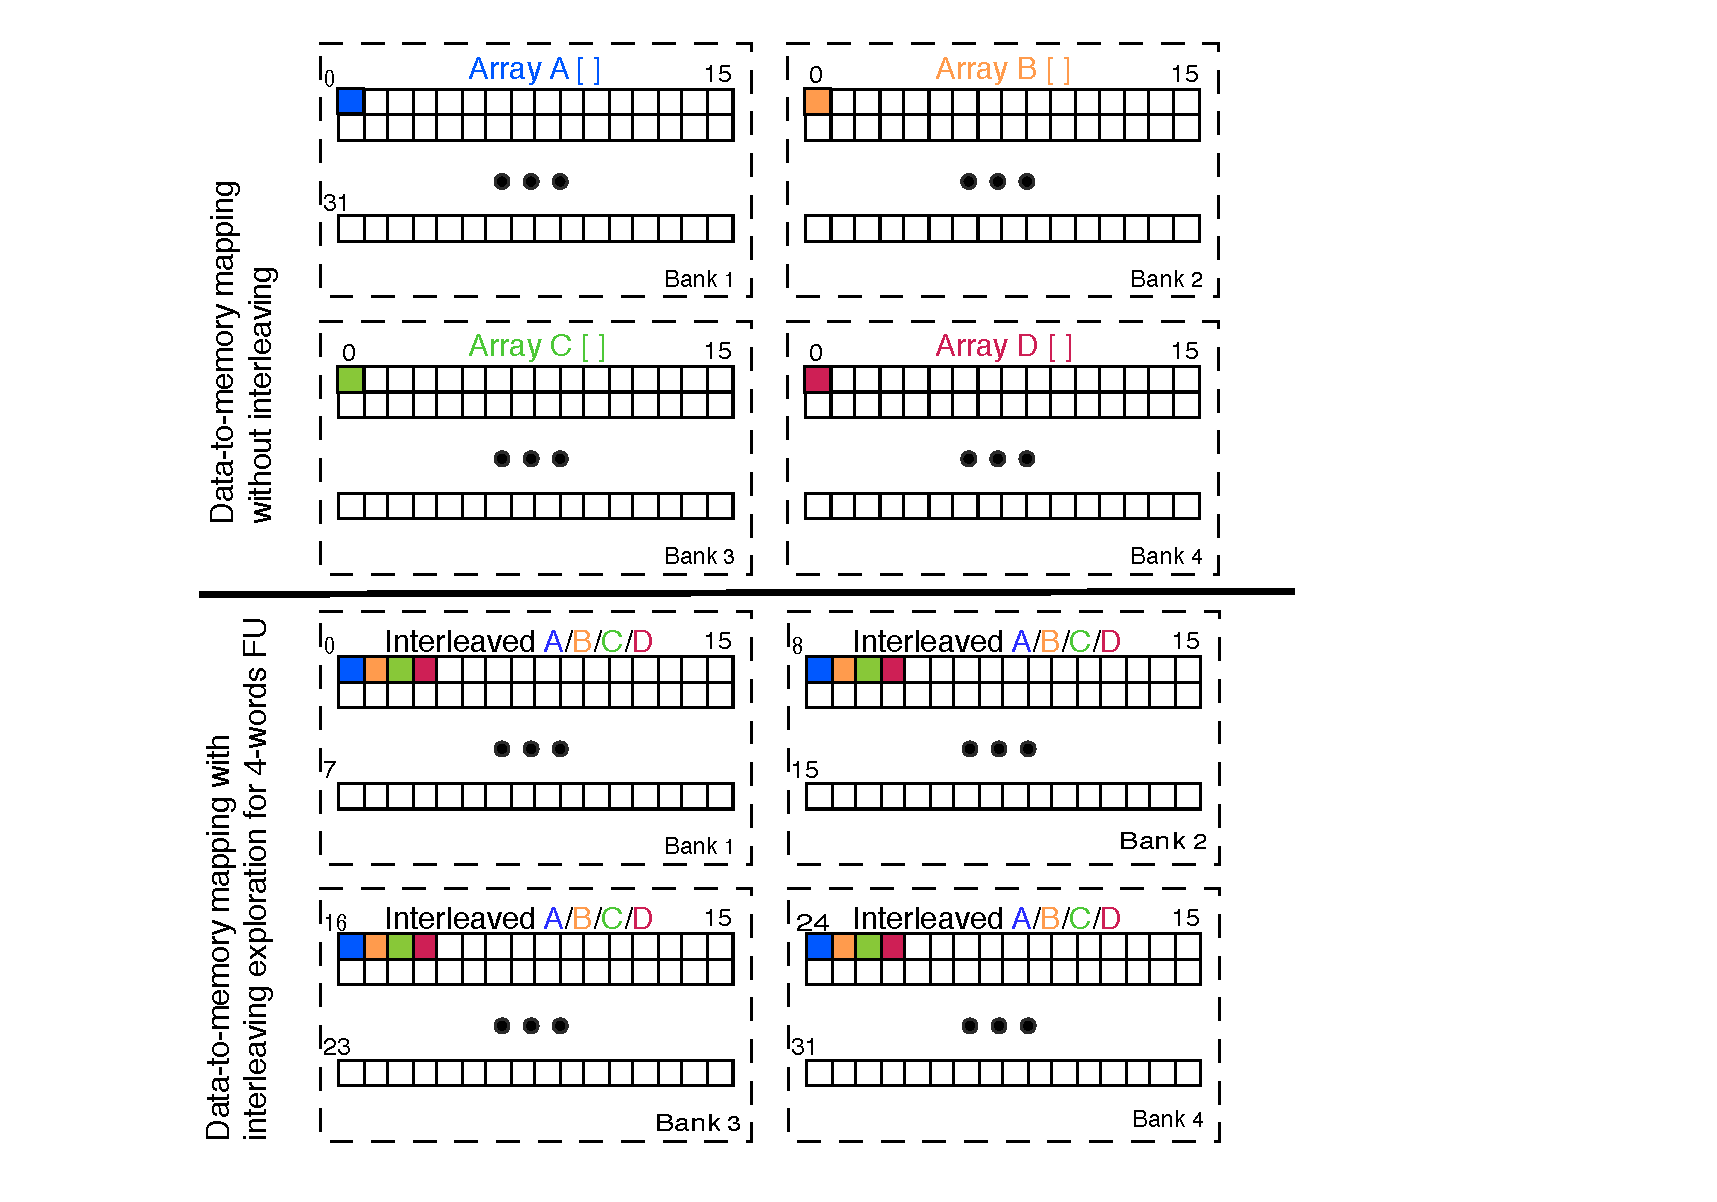
\includegraphics[scale = 0.5]{Images/motivation.eps}
\end{figure}

A quick estimation for the difference in the energy consumption between the two approaches can be calculated using a simple energy model for the system.
The system architecture has an ADD FU that performs operations over 4 words at a time and the memory to processor path has a width of 4 words. 
Each array element is assumed to have the size of one word.
The register file at the processor can only store 5 words and the iteration variable $i$.
The first approach 

\section{Related work}



\section{System Design Exploration Workflow}

The general workflow of this work is presented in Fig.\ref{workflow}.

\begin{figure}
\centering
	\label{workflow}
	\caption{Methodology steps}
	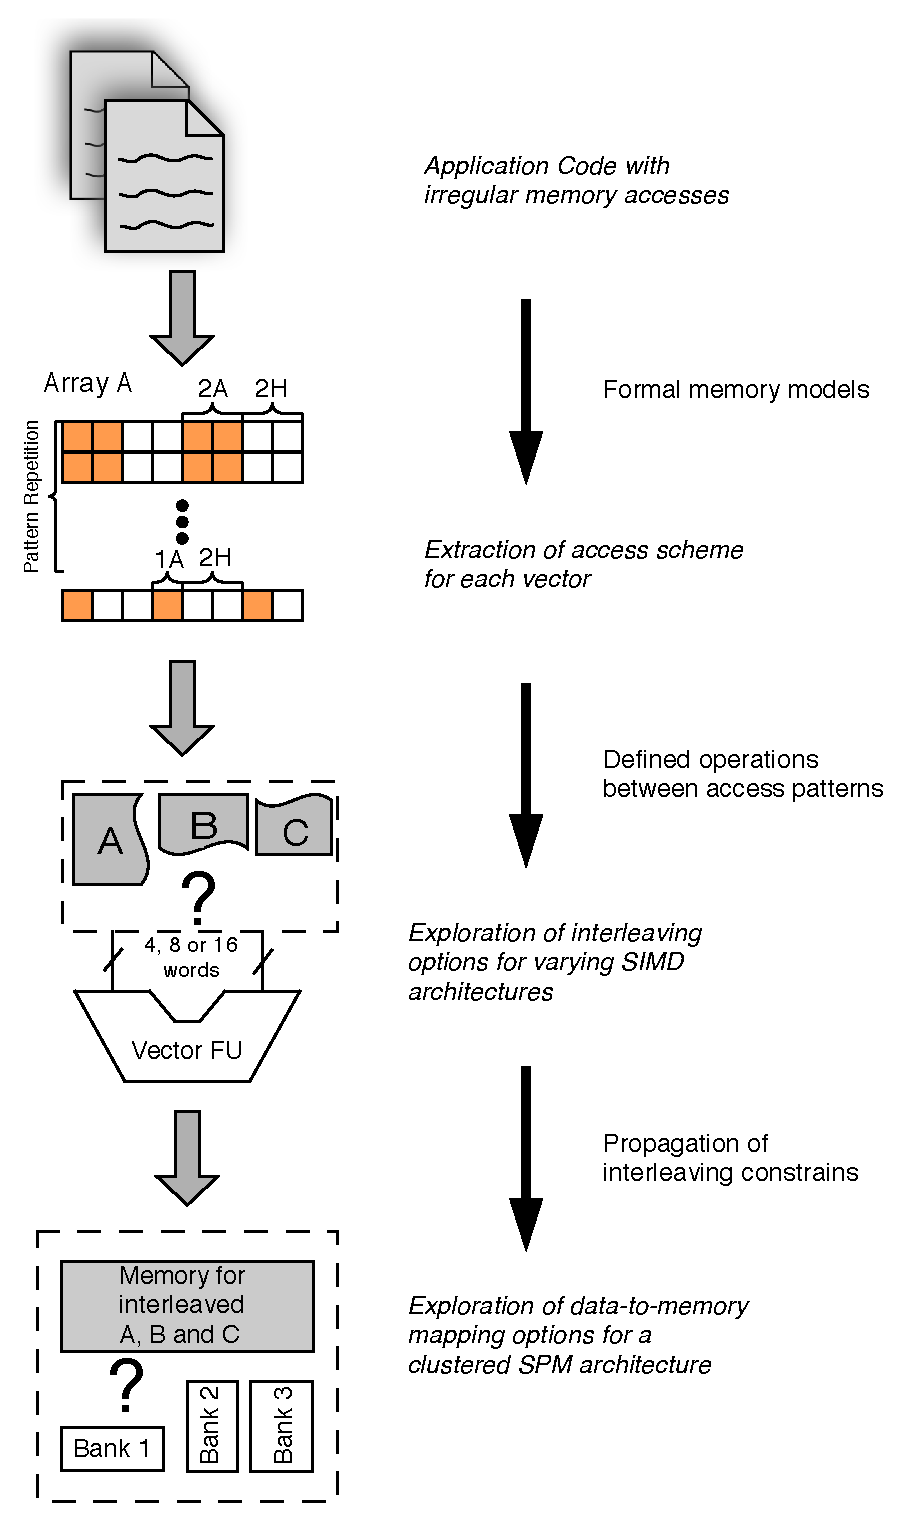
\includegraphics[scale = 0.5]{Images/Workflow.eps} 
\end{figure}

\subsection{Formal Model Representation of Access Pattern }

A representation model for the access pattern is employed in order to formally present each step of the methodology.

\textit{Discussion about polyhedral and enumerative approaches}

\textit{Analysis of A-H model based on Angeliki}

\textit{Definition of algebra functions between access patterns}

\subsection{Data Interleaving Exploration}

\textit{Algorithm for exploring data interleaving}

\subsection{Data-to-Memory Mapping Exploration}

Given the input from the previous step, we explore the mapping of data-to-memory.

\subsection{One way constraint propagation}

The decisions taken on the interleaving step affect the mapping options.
If the interleaving decisions lead to small compact sets of data, the mapping can be done on small energy efficient memory banks.
On the other hand, if the mapping exploration is performed first, the freedom for interleaving is reduced.
We split the decisions in two steps and the interleaving decisions are propagated as constraints on the mapping exploration phase. 

\section{Target Architecture}

\textit{Analysis of architecture based on our previous papers}

General architecture is presented in Fig.\ref{arch}.

\begin{figure}
\centering
	\label{arch}
	\caption{Exploration options and system knobs depending on a general platform architecture}
	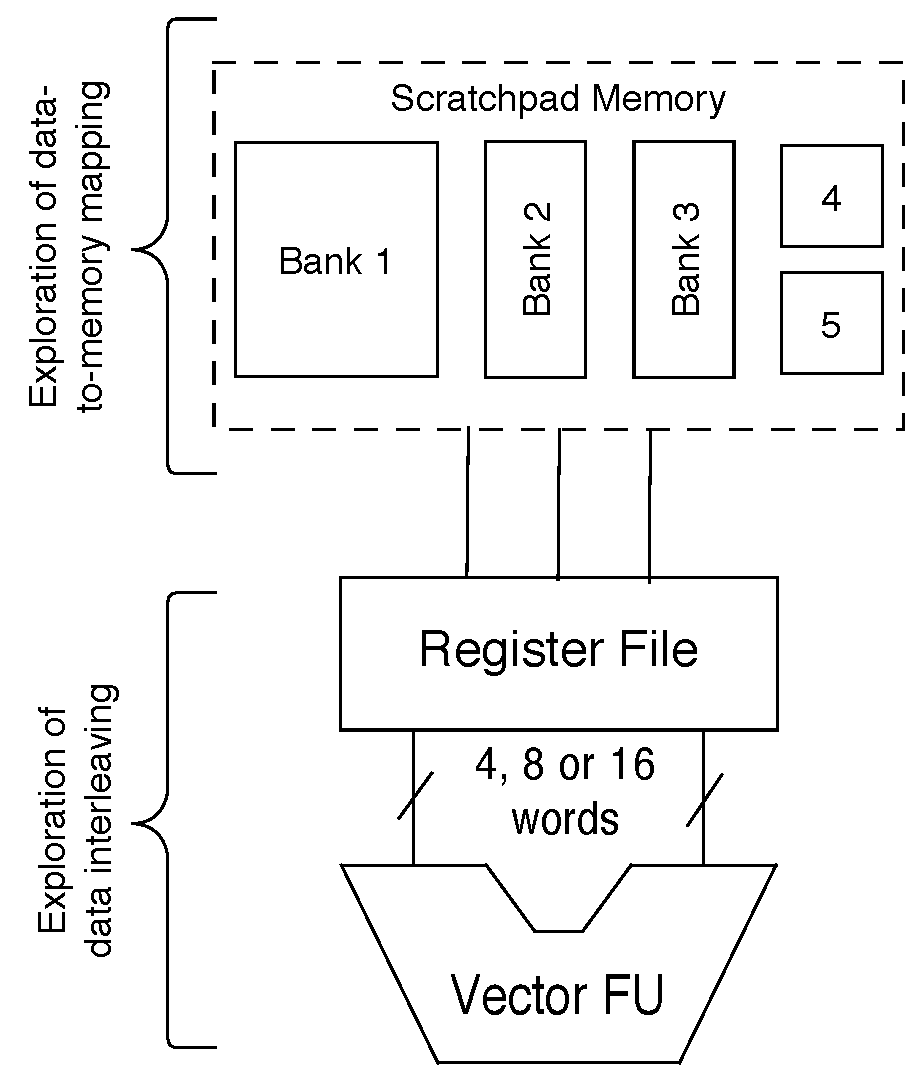
\includegraphics[scale = 0.5]{Images/Architecture.eps} 
\end{figure}

\section{Applications}

An example of the channel estimation kernel is presented in Fig. .

Suitable applications:
\begin{itemize}
\item Channel estimation kernel
\item SOR benchmark
\item Motion estimation kernel
\item PGM-armor
\item Maybe image processing...
\end{itemize}

\section{Results}


\begin{table}%
\tbl{Normalized energy consumption\label{tab:results}}{
\begin{tabular}{c c}
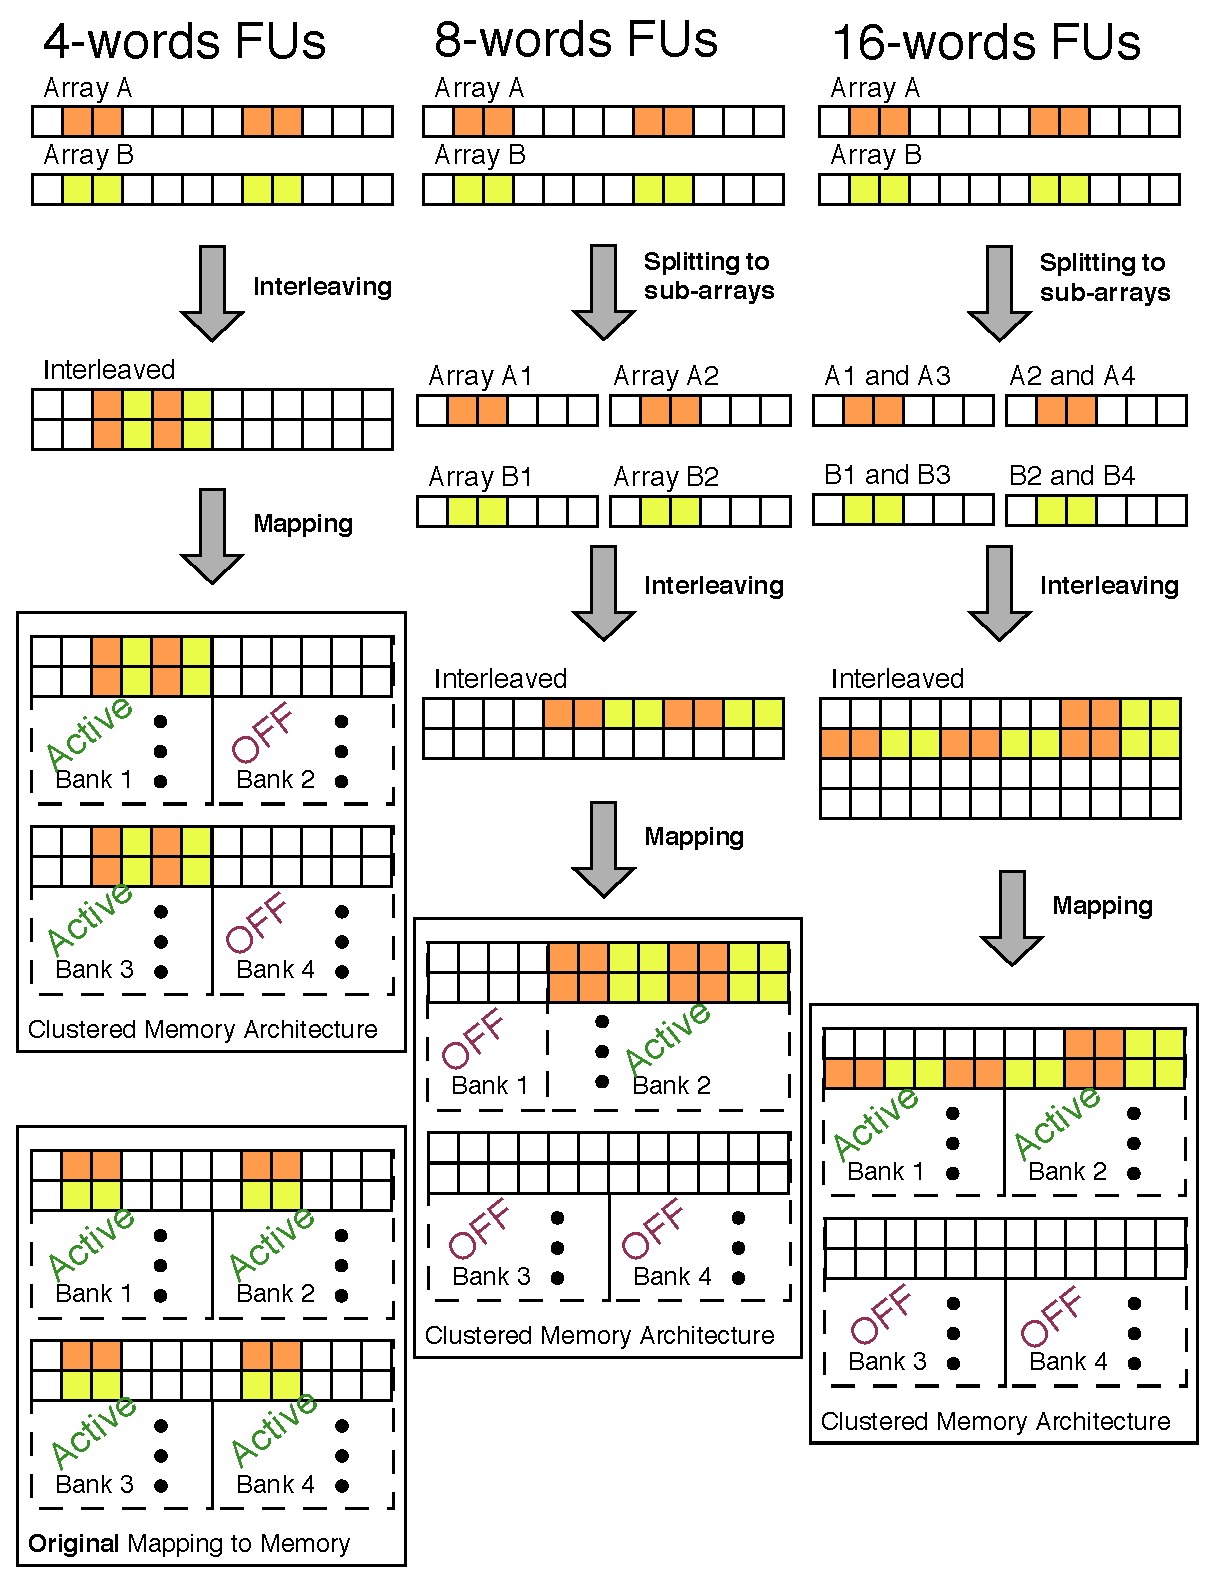
\includegraphics[width=0.45\linewidth]{Images/Example.eps} & 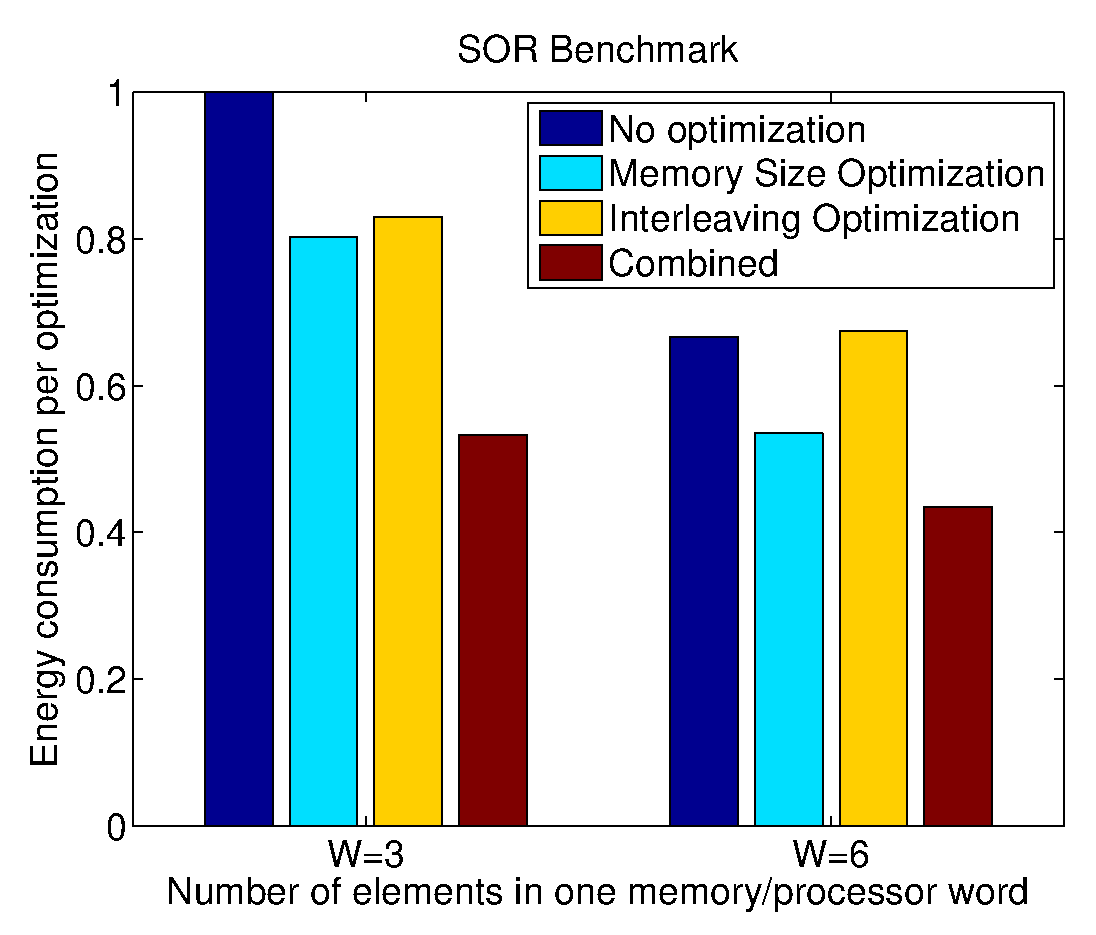
\includegraphics[width=0.45\linewidth]{Images/sor.eps} \\
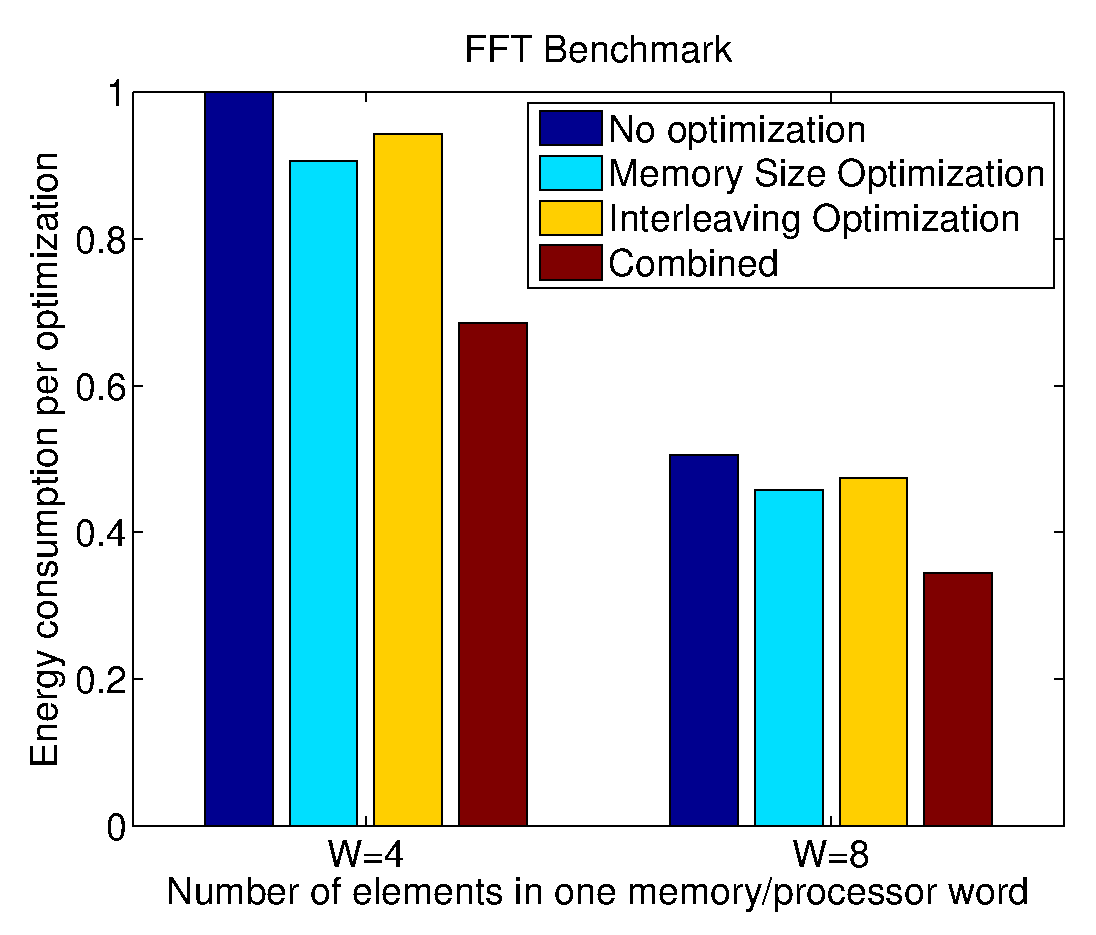
\includegraphics[width=0.45\linewidth]{Images/fft.eps} & 
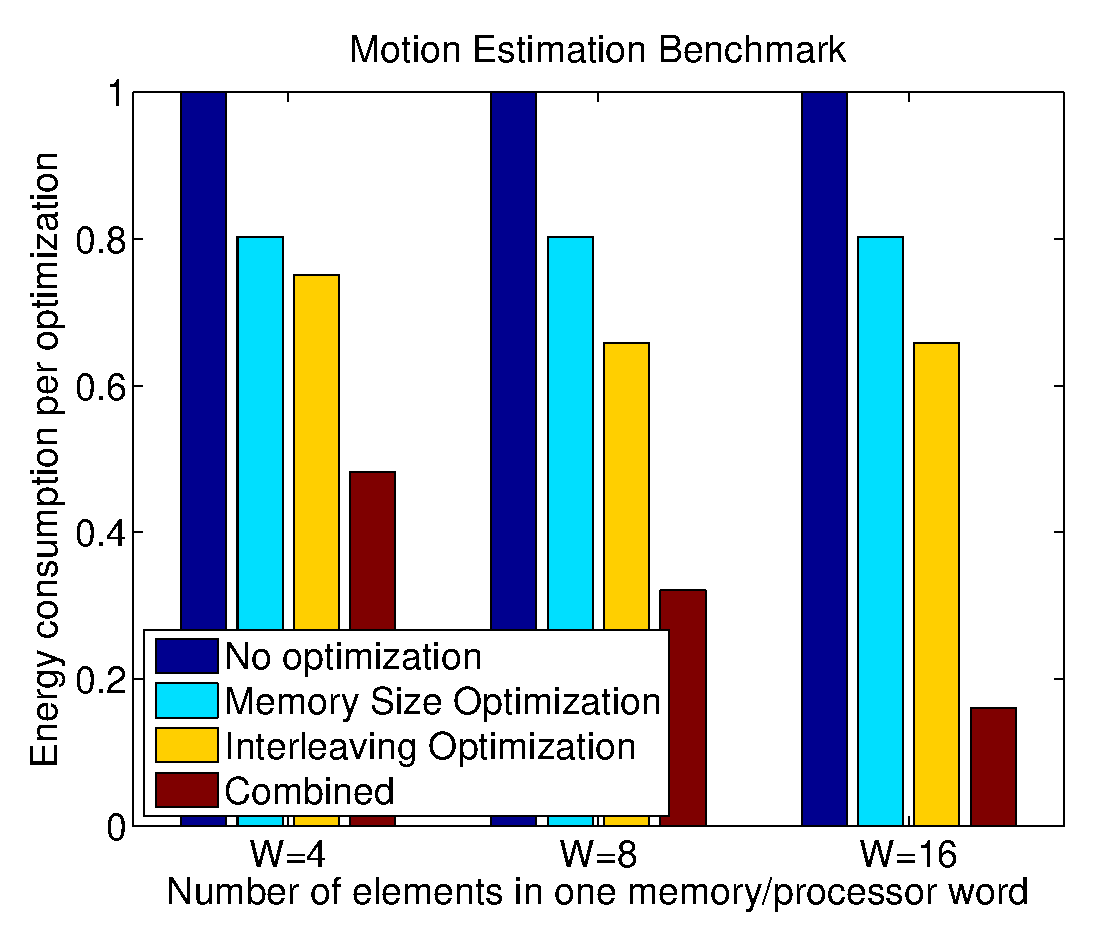
\includegraphics[width=0.45\linewidth]{Images/mest.eps} 
\end{tabular}}
\end{table}


The design exploration is applied to the chosen application benchmark and energy numbers are derived based on the described target platform.
Results are presented for the four cases:
\begin{itemize}
\item No optimization
\item Interleaving exploration with a static memory platform (gain A)
\item Data mapping exploration on a reconfigurable platform without optimized interleaving (gain B)
\item Co-exploration of interleaving and mapping options (gain C, C$ > $A+B )
\end{itemize}

% Bibliography
\bibliographystyle{ACM-Reference-Format-Journals}
\bibliography{reference}

\end{document}